\paragraph{Цель работы}
Эта лабораторная работа проведёт вас через все этапы построения законченного приложения на Qt. Целью является понимание структуры приложения на Qt и получение опыта использования стандартной документации Qt.

\paragraph{Задание}
Написать текстовый редактор со следующим функционалом:
\begin{itemize}
    \item Копирование, вставка, отмена и повторение действий
    \item Открытие файла, его сохранение
    \item Изменение шрифта
    \item Оповещение при выходе без сохранения.
\end{itemize}

\lstinputlisting[language=C++]{../../src/QT/2/text_editor/mainwindow.h}
\lstinputlisting[language=C++]{../../src/QT/2/text_editor/mainwindow.cpp}

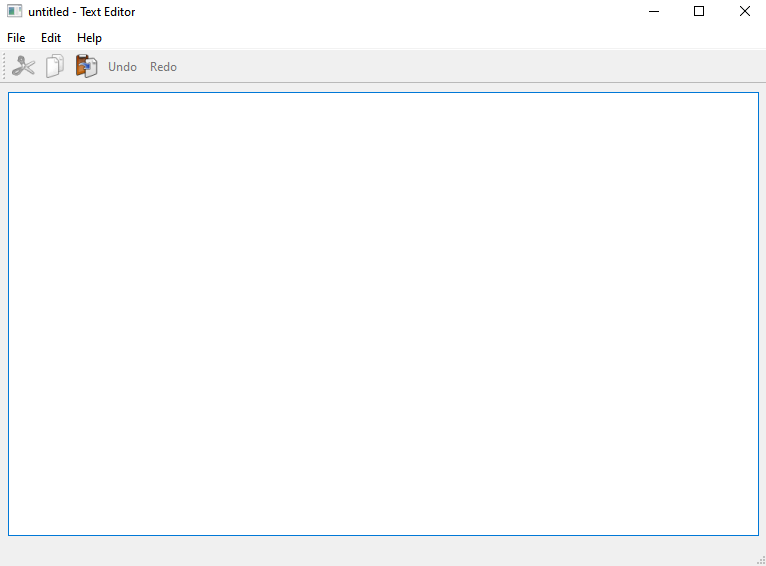
\includegraphics[width=0.6\textwidth]{scr1.PNG}

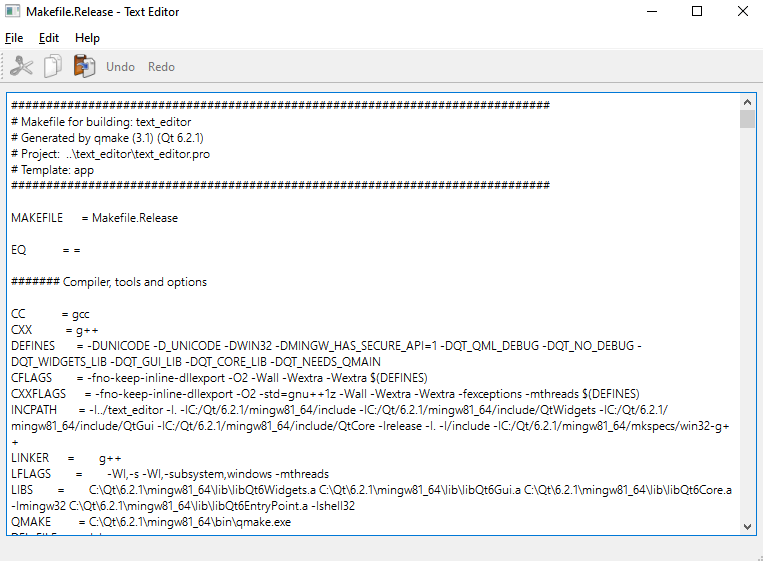
\includegraphics[width=0.6\textwidth]{scr2.PNG}

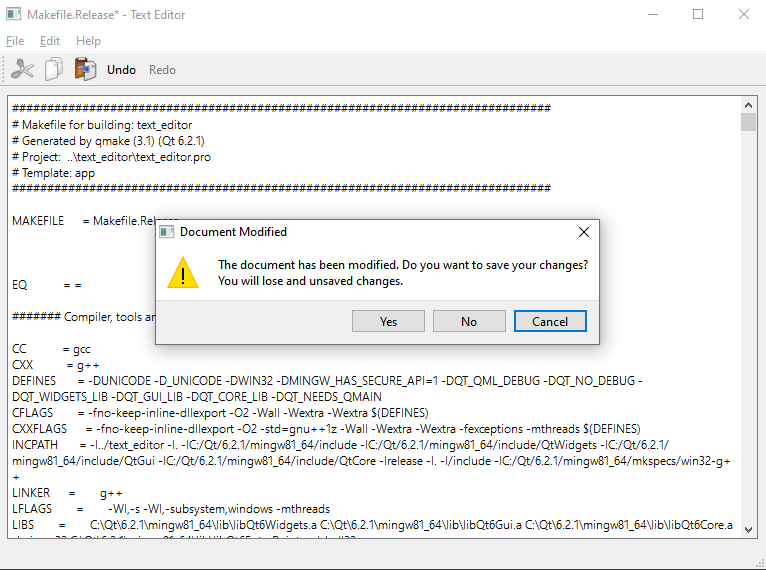
\includegraphics[width=0.6\textwidth]{scr3.PNG}


\includegraphics[width=0.6\textwidth]{scr4.PNG}

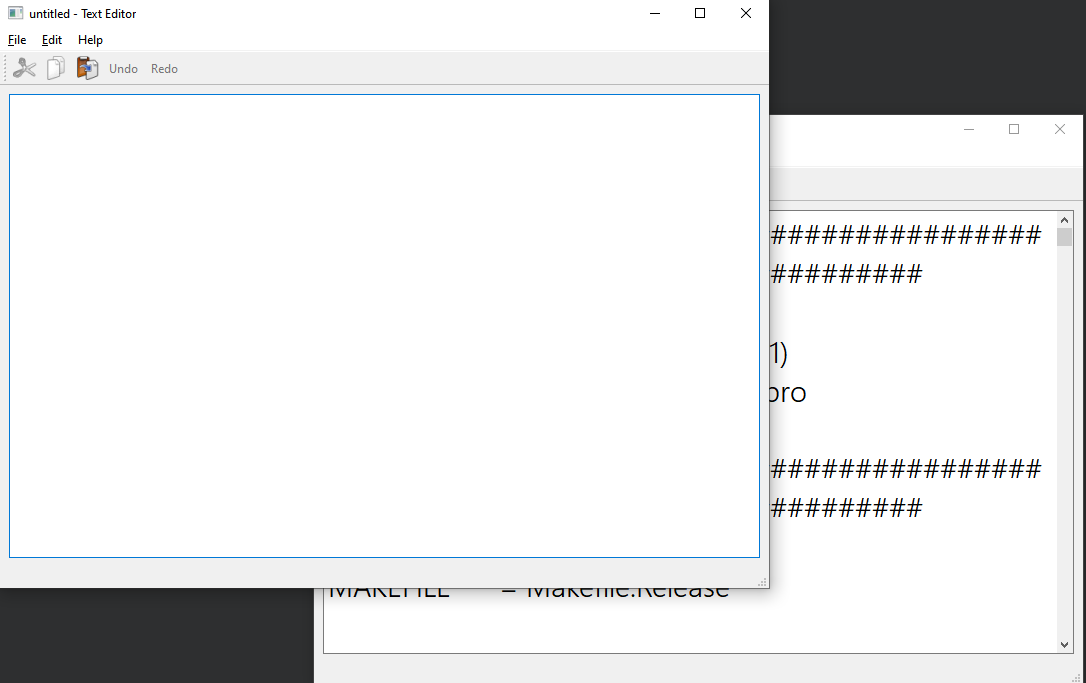
\includegraphics[width=0.6\textwidth]{scr5.PNG}